%
% File acl2015.tex
%
% Contact: car@ir.hit.edu.cn, gdzhou@suda.edu.cn
%%
%% Based on the style files for ACL-2014, which were, in turn,
%% Based on the style files for ACL-2013, which were, in turn,
%% Based on the style files for ACL-2012, which were, in turn,
%% based on the style files for ACL-2011, which were, in turn, 
%% based on the style files for ACL-2010, which were, in turn, 
%% based on the style files for ACL-IJCNLP-2009, which were, in turn,
%% based on the style files for EACL-2009 and IJCNLP-2008...

%% Based on the style files for EACL 2006 by 
%%e.agirre@ehu.es or Sergi.Balari@uab.es
%% and that of ACL 08 by Joakim Nivre and Noah Smith

\documentclass[11pt]{article}
\usepackage{acl2015}
\usepackage{times}
\usepackage{url}
\usepackage{latexsym}
\usepackage{graphicx}
% \usepackage{cite}  


%\setlength\titlebox{5cm}

% You can expand the titlebox if you need extra space
% to show all the authors. Please do not make the titlebox
% smaller than 5cm (the original size); we will check this
% in the camera-ready version and ask you to change it back.


\title{Combining Graph Convolutional Network and Transformers for Multimodal Sentiment Analysis}

\author{
  Wanrong Zheng,
  Xinwei Du,
  Haosheng Wang
  }
  
\date{\today}

\begin{document}
\maketitle
% \begin{abstract}
%   This document contains the instructions for preparing a camera-ready
%   manuscript for the proceedings of ACL-2015. The document itself
%   conforms to its own specifications, and is therefore an example of
%   what your manuscript should look like. These instructions should be
%   used for both papers submitted for review and for final versions of
%   accepted papers.  Authors are asked to conform to all the directions
%   reported in this document.
% \end{abstract}

\section{Problem Definition}
Multimodal sentiment analysis is the task of performing sentiment analysis given multiple data sources (vision, audio, language).
A good understanding of this task can help us better understand human social behavior and benefit human-computer interaction since human communication is multimodal and emotional.
Latest Deep Learning techniques allow us using novel approaches to utilize these different types of signals into one model to form joint feature.  


\section{Literature Review}
\noindent \textbf{Feature Fusion:}
Multiple models have been proposed to consider the multi-modality fusion. \cite{DBLP:journals/corr/VaswaniSPUJGKP17} proposes Sentiment Inference Subnetwork conditioned on the output of the Tensor
Fusion Layer and performs sentiment inference. 
\cite{DBLP:journals/corr/abs-1802-00927} presents a new neural architecture for multi-view sequential learning called the Memory Fusion Network that explicitly accounts for both interactions in a neural architecture and continuously models them through time.
\cite{bagher-zadeh-etal-2018-multimodal} proposes a novel multimodal fusion technique called the Dynamic Fusion Graph (DFG), which conduct experimentation to exploit how modalities interact with each other in human multimodal language and is highly interpretable.

\noindent \textbf{Recent Progress:}
In the previous research, \cite{DBLP:journals/corr/abs-2006-15955} proposes a state-of-the-art approach to this topic. This approach describes a Transformer-based\cite{DBLP:journals/corr/VaswaniSPUJGKP17} joint-encoding for the task of Emotion Recognition and Sentiment Analysis. 
This approach uses a new encoding architecture that fully eschews recurrence for sequence encoding and instead relies entirely on an attention mechanism and Feed-Forward Neural Networks to draw global dependencies between input and output. Its results can compare with, and sometimes surpass, the current state-of-the-art for both tasks on the CMU-MOSEI dataset.
However, such a network directly computes each task separately and combine them to a joint-encoding which ignores the connections between multimodel.
Therefore, we are going to build a model which combines Graph Convolutional Network (GCN) \cite{DBLP:journals/corr/KipfW16} and Transformers encoding.

\section{Method}
\subsection{Transformer}

\subsection{Similarity Network}

\subsection{GCN}

We want to use the graph convolutional network to handle the multimodal sentiment analysis task.

\subsubsection{Preliminaries of the GCN}

Given the dataset $D = \{d_1,\cdots,d_n \}$, where $d_i$ is the input data which consists of three different modalities (visual, audio and language). We can use the neural network or manually defined rules to extract features. For example, we can extract facial action units from the visual modality, we can extract MFCCs from the audio modality and we can use glove word embedding to represent features extracted from the language modality.

Let $X = \{x_1,\cdots,x_n \}$ be the extracted features from the raw dataset $D$. Given the extracted features $X$ , we can use an adjacency matrix $A$ to represent the relationship between data. $A_{ij}$ represent the relationship between data $d_i$ and data $d_j$. We can set $A_{ij} = N(x_i, x_j)$ if data $d_i$ and data $d_j$ have relationship. $N(\cdot,\cdot)$ is the function to calculate the similarity of two data given the features extracted from those two data. 

Given the adjacency matrix $A$ and extracted features $X$, we can define a graph $G = (X, A)$. This graph is the key component of the GCN algorithm. Equation (\ref{eq1}) shows a simplified architecture of the GCN proposed by \cite{kipf2017semi}.

\begin{equation}
X^{(l+1)}=\sigma (LX^{(l)}W^{(l)})
\label{eq1}
\end{equation}

In Equation (\ref{eq1}), $X^{(l)}$ is the features of the data in the $l$th layer of the network.
When $l = 1$, $X^{(1)}$ is the features we extracted from the data. When $l>1$, $X^{(l)}$ is learned by the GCN.
$W^{(l)}$ is a trainable weight of the $l$th layer of the graph convolution network.
Matrix $L$ is the graph filter. $L$ is not a trainable variable, it represents property of the graph $G$. The definition of the graph filter $L$ varies, which can be different depending on the tasks. One standard definition of $L$ is let $L = A$. Therefore, the graph filter $L$ times features $X^{(l)}$ means that each nodes' features in $l+1$th layer are related to its neighbors' features in $l$th layer.

In our method, we use Equation (\ref{eq2}) and (\ref{eq3}) to calculate the graph filter $L$.
This method is proposed by \cite{kipf2017semi}. 
The eigenvalues of $L$ calculated in this way are limited to (-1,1]. It can prevent the 
gradient vanishes and gradient explodes problems in multi-layer GCN.

\begin{equation}
\bar{A}= A + I
\label{eq2}
\end{equation}

\begin{equation}
L_{ij}=\frac{\bar{A}_{ij}}{\sqrt{\sum_{m=1}^{n} \bar{A}_{im}}
\sqrt{\sum_{m=1}^{n} \bar{A}_{mj}}} 
\label{eq3}
\end{equation}

\subsubsection{Training}
We first select some data $D_{sub}$, for example, 128 different videos, from the dataset $D$. Next, we can get the extracted features $X_{sub}$ 
(such as facial action units, MFCCs, word embedding, etc.) from those videos $D_{sub}$.

We use function $N(\cdot,\cdot)$  to calculate the adjacency matrix $A$ and use Equation (\ref{eq2}) and (\ref{eq3}) to calculate the graph filter $L_{sub}$. We can build a multi-layer GCN according to Equation (\ref{eq1}). The input of the GCN is the data features $X_{sub}$ and the graph filter $L_{sub}$. In one round of training, the graph filter $L_{sub}$ in different GCN layers is the same. And $L_{sub}$ is different in different training round since $L_{sub}$ represents the relationship between data in $D_{sub}$.

The output of the GCN is $X_{sub}^{l}$, which represents the relearned features of the data. We can use those features to further do classification or regression tasks. For example, we can simply use a full connection layer to predict the result.

\subsubsection{Referencing}

Given a video $d_{test}$ needed to be predicted, we can select several videos from the training set, and get the video set $D_{sub}$. The following part is the same as the training part. We extract $X_{sub}$, construct $L_{sub}$, use GCN to get the relearned features of $X_{sub}$, and use the relearned features to do the classification or regression tasks.


\section{Experiments}

\subsection{Dataset}

Considering that the multimodal model can perform sentiment analysis from different perspectives such as images, sounds, and texts, the following datasets will be more in line with the requirements of this paper.

\textbf{CMU Multimodal Opinion Sentiment and Emotion Intensity (CMU-MOSEI)}  dataset is the largest dataset of multimodal sentiment analysis and emotion recognition to date. The dataset contains more than 23,500 sentence utterance videos from more than 1000 online YouTube speakers. The dataset is gender balanced. All the sentences utterance are randomly chosen from various topics and monologue videos. The videos are transcribed and properly punctuated.The following Figure.\ref{fig:SSN} gives an overview of the dataset statistics:

\begin{figure}[t] % picture
    \centering
    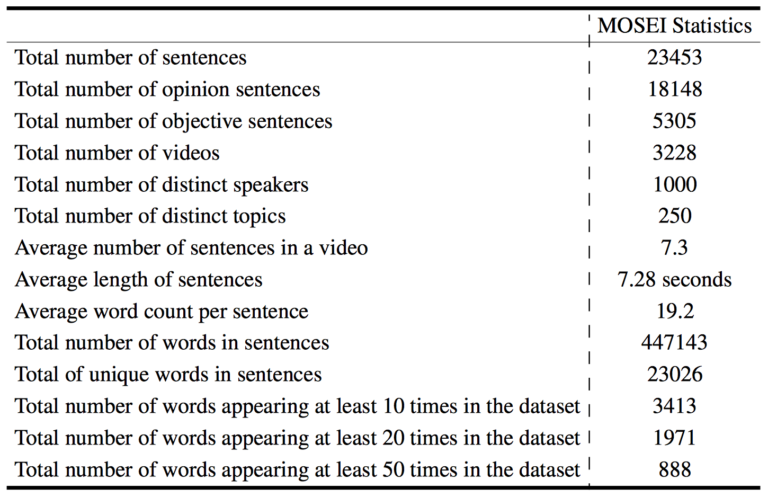
\includegraphics[width=\columnwidth]{img/mosei.png}
    \caption{Overview of the CMU-MOSEI dataset statistics. Demonstrated the details of sentences.}
    \label{fig:SSN}
\end{figure}

\textbf{CMU-MOSI} dataset is a collection of 2199 opinion video clips. Each opinion video is annotated with sentiment in the range [-3,3]. The dataset is rigorously annotated with labels for subjectivity, sentiment intensity, per-frame and per-opinion annotated visual features, and per-milliseconds annotated audio features.

\subsection{Experiment setup}

\subsection{Results}

\begin{table}[t]
\centering
%\begin{tabular}{cc}
%\begin{minipage}{.5\linewidth}
%\centering
\begin{tabular}{ll}
\hline
\textbf{Methods}       & \textbf{Accu}      \\ 
\hline
Transformer-based joint-encoding & 82.40      \\ 
Multilogue-Net & 82.10     \\ 
B2 + B4 w/ multimodal fusion & 81.14     \\ 
Our Transformer-based baseline  & \textbf{80.13} \\ 
CAE-LR & 78 \\
Graph-MFN & 76.9 \\
MFN & 76.0 \\ \hline
\end{tabular}
\caption{\label{result}Comparison with related methods on CMU-MOSEI}
\end{table}


\section{Conclusion}

\section{Team Member Contributions}

\quad Xinwei Du: Read articles about fusion algorithms. Data exploration. Focusing on how to build a graph for GCN.

Wanrong Zheng: Survey for baseline and benchmark. Design on the ablation study of building one GCN graphs each modality and different ways to construct edges. Implement the swin-transformer structure.

Haoshen Wang: Data collecting. Establish the baseline model. Focusing on graph fusion.

% include your own bib file like this:
\bibliographystyle{acl}
\bibliography{ref}


\end{document}